\documentclass[10pt,twocolumn,letterpaper]{article}
\usepackage[review]{cvpr}
\usepackage{tikz,pgfplots}
\pgfplotsset{compat=1.18}
\usepackage[T1]{fontenc}
\usepackage{times,amsmath,amssymb,graphicx,booktabs,multirow,array,xcolor}
\usepackage[pagebackref,breaklinks,colorlinks,allcolors=blue]{hyperref}
\usepackage[capitalize]{cleveref}
\def\confName{CVPR}\def\confYear{2027}
\title{Beyond Processing Artifacts: Controlled Evaluation and Training\\for Single-Image Morphing Attack Detection}
\author{Anonymous submission}
\begin{document}
\maketitle
\begin{abstract}
A face morph detector can separate benchmark morphs from genuine photographs without detecting the combination of two identities. We investigate this ambiguity through morph-free training, matched manipulation controls, and training ablations. Networks trained only to distinguish synthetic faces from shrink-and-enlarge copies achieve zero equal error rate on the native MorDIFF evaluation in all ten tested networks. We introduce comparisons that progressively control rendering, warping, blending, and contributor identity, revealing substantial responses to single-photo reconstructions and no established advantage beyond low-level statistics in a matched blend-versus-warp diagnostic. We then study training with face-spliced morphs and matched same-person and seam-only negatives. A count-balanced development ablation improves two-person versus same-person ranking by 0.048 AUC across five seeds; negative content remains confounded with 312 additional unique images. The full protocol attenuates storage-induced false alarms. The development-exposed MAD22 comparison establishes neither superiority nor morph-specific detection. Together, the results provide an evaluation framework and a qualified training benefit while identifying the evidence still needed for identity-specific detection.
\end{abstract}

\section{Introduction}
Face morphing attacks~\cite{ferrara2014magic} exploit photographs combining contributors. A single-image detector can instead recognize acquisition, resampling, blending, reconstruction or storage traces. Morph-versus-photograph accuracy alone cannot distinguish processing sensitivity from identity-specific detection, even when performance transfers between engines.

We test this ambiguity with morph-free training and matched controls. All ten networks trained to recognize shrink-and-enlarge copies of synthetic faces achieve zero EER on native MorDIFF~\cite{damer2023mordiff} under our preprocessing. This establishes processing-cue sufficiency for that cell, not a common mechanism across detectors or blur as the unique cause. Single-photo reconstructions, warp-only images and same-person manipulations then control progressively more of the construction; low-level differences can nevertheless remain.

Finally, a count-balanced development follow-up supports improved ranking in the full splice-positive recipe, controlling rows, classes and positive repetition within pairs. Negative content remains confounded with image diversity; the analogous pair without splice positives lacks the registered benefit. Blend-versus-warp and reconstruction controls retain important limitations.

Our contributions are:
\begin{enumerate}
\item A processing-cue audit showing that a morph-free training task can attain perfect separation on a morph benchmark cell, supported by paired processing and single-photo reconstruction controls.
\item A controlled evaluation framework separating questions about rendering, warping, blending, and contributor identity, with explicit limits on what each contrast establishes.
\item A matched-control training study showing a count-balanced development ranking gain in the full recipe, with content and image diversity still confounded, alongside attenuated storage false alarms and a qualified benchmark comparison.
\end{enumerate}

\begin{figure*}[t]
\centering
\ifdefined\UsePlotlyFigures
\includegraphics[width=\textwidth]{figures/plotly_js/controls_overview_js.pdf}
\else
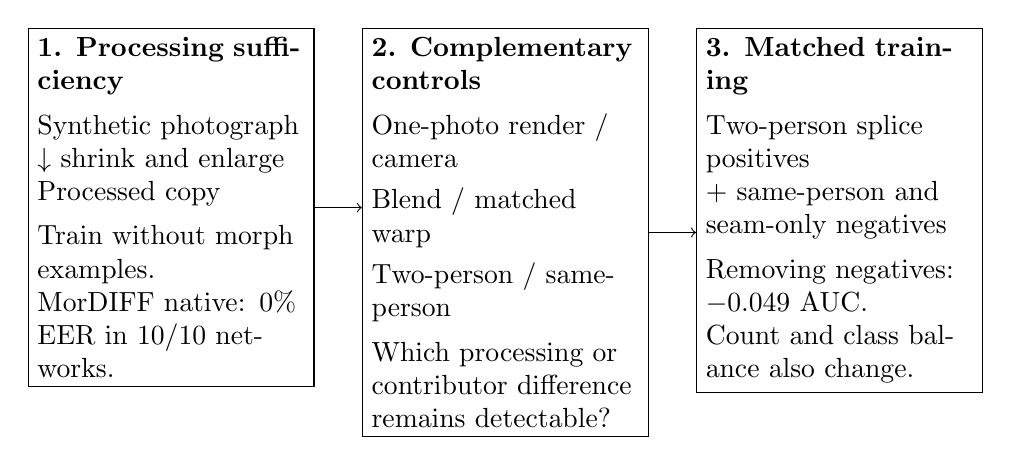
\begin{tikzpicture}
\node[draw,text width=.28\textwidth,align=left,anchor=north west] (a) at (0,0) {
\textbf{1. Processing sufficiency}\\[4pt]
Synthetic photograph\\
$\downarrow$ shrink and enlarge\\
Processed copy\\[4pt]
Train without morph examples.\\
MorDIFF native: 0\% EER in 10/10 networks.};
\node[draw,text width=.28\textwidth,align=left,anchor=north west] (b) at (.35\textwidth,0) {
\textbf{2. Complementary controls}\\[4pt]
One-photo render / camera\\[3pt]
Blend / matched warp\\[3pt]
Two-person / same-person\\[4pt]
Which processing or contributor difference remains detectable?};
\node[draw,text width=.28\textwidth,align=left,anchor=north west] (c) at (.70\textwidth,0) {
\textbf{3. Matched training}\\[4pt]
Two-person splice positives\\
$+$ same-person and seam-only negatives\\[4pt]
Removing negatives: $-0.049$ AUC.\\
Count and class balance also change.};
\draw[->] (a.east) -- (a.east -| b.west);
\draw[->] (b.east) -- (b.east -| c.west);
\end{tikzpicture}

\fi
\caption{The experimental argument (conceptual schematic). Morph-free training establishes processing-cue sufficiency on native MorDIFF under the tested preprocessing. Controls ask narrower questions about rendering, warping, blending and contributor identity. The original removal ablation changes count and class balance; its count-balanced follow-up still confounds negative content with image diversity.}
\label{fig:argument}
\end{figure*}

\section{Related Work}
\label{sec:related}

\paragraph{Morph generation and attack detection.}
Face morphing exploits the possibility that a single enrollment image can resemble multiple contributors, illustrated by the passport attack of Ferrara et al.~\cite{ferrara2014magic}. The SYN-MAD competition evaluates transfer from synthetic training data to real-image attacks~\cite{huber2022synmad}; SMDD established synthetic-only MAD training~\cite{damer2022smdd}. Generation methods differ substantially in how this resemblance is constructed. MIPGAN introduces identity constraints into GAN-based synthesis~\cite{zhang2021mipgan}, whereas MorDIFF uses diffusion autoencoders for representation-level interpolation~\cite{damer2023mordiff}. These mechanisms introduce different reconstruction and processing histories in addition to changes in identity content. Consequently, detecting images produced by a morphing pipeline and detecting evidence attributable to two identities are distinct empirical questions. Our comparisons retain conventional morph-versus-photo evaluation but add controls that hold more of the construction process in common. We do not assume that a shared generator eliminates all low-level differences, nor that an image involving two people necessarily constitutes a successful recognition attack.

\paragraph{Foundation models and synthetic supervision.}
CLIP learns transferable representations through image--text supervision~\cite{radford2021clip}; LoRA adapts pretrained weights using trainable low-rank updates~\cite{hu2022lora}. Their use for morph detection precedes this work. In particular, MADation adapts CLIP with LoRA and a binary classification head~\cite{caldeira2025madation}. Our contribution therefore concerns training examples, controlled evaluation, and the interpretation of detector responses, rather than a new foundation-model architecture. Holding the backbone and optimization recipe fixed allows comparisons of alternative training lists, although removing examples can still change class balance, repetition, and effective diversity. These quantities must be accounted for before attributing an effect specifically to the semantic content of the added controls.

SelfMAD addresses cross-method generalization through self-supervised simulation of morphing artifacts in pixel and frequency space~\cite{ivanovska2025selfmad}. This is closely related to the use of synthetic supervision, but it also highlights a central question for evaluation: which simulated artifacts remain specific to an attack when acquisition and processing change? SelfMAD++ combines such augmentation with a CLIP-based model, local spatial features, and auxiliary segmentation~\cite{ivanovska2026selfmadpp}. We distinguish these two methods; evaluation of the released SelfMAD detector does not establish superiority over SelfMAD++. Our approach is complementary to architecture and augmentation improvements: paired controls can be used to examine their decision mechanisms without presuming that any particular training strategy is inherently artifact-independent.

\paragraph{Shortcut learning and mechanistic evidence.}
Geirhos et al.~\cite{geirhos2020shortcut} describe shortcut learning as the use of predictive rules that succeed under benchmark conditions but fail under more challenging conditions. In morph detection, processing history is a plausible source of such prediction because the two classes can differ systematically in resampling, storage, reconstruction, or image boundaries. A strong benchmark result alone cannot distinguish these explanations from sensitivity to identity mixing. Conversely, a processing perturbation that changes a detector's output does not prove that processing explains every correct decision.

This concern also has direct MAD precedent. A recent print--scan study reports substantial degradation of digitally trained detectors across acquisition devices~\cite{paulo2026printed}. Our storage and reconstruction controls ask a complementary question: can processing produce an attack response even when no second identity is present? This complements domain-shift evaluation with matched tests of score specificity.

\paragraph{Blending as supervision and as a control.}
Face X-ray learns a representation of blending boundaries for general face-forgery detection~\cite{li2020facexray}. Self-Blended Images synthesize forgery supervision by blending transformed versions of a single pristine image~\cite{shiohara2022sbi}. Both establish that useful manipulation supervision can be generated without examples from the target forgery method. Their objective is to recognize forgery traces; our same-person and seam-only negatives instead challenge the sufficiency of selected traces for a two-contributor label. A self-blend can therefore be a useful positive for forgery detection and a useful negative control for contributor dependence. This difference in target property, rather than a claim that blending artifacts are universally undesirable, motivates our construction.

Our contribution connects three tests: processing-only supervision as a benchmark counterexample, matched comparisons that separate rendering and blending from contributor changes, and a controlled study of adding matched negatives. The framework tests whether a proposed explanation survives a specified comparison. It neither introduces a new backbone nor certifies an identity mechanism; texture, noise averaging, geometry and the surround remain measurable alternative explanations.

\section{Controlled Evaluation of Morph Detection}
\label{sec:controls}

A detector can separate benchmark morphs from genuine photographs without identifying the property that motivates the task: contributions from different people. Our framework therefore asks two questions separately: which image transformations are sufficient to activate a detector, and whether discrimination persists when the negative example undergoes a comparable construction process. We use the term \emph{control} for an image that removes a proposed explanation from a comparison. It does not imply that every control is an unmodified bona fide photograph.

\subsection{Image processing and identity mixing}
Let $x_i$ denote a photograph of person $i$, and let $x'_i$ be a different photograph of the same person. Write $M_e(x_i,x_j)$ for an image produced by morphing engine $e$, and $P_h(x)$ for an image with processing history $h$. A conventional comparison separates $M_e(x_i,x_j)$, $i\ne j$, from $x_i$. Its class difference includes identity mixing, geometric warping, blending, rendering, storage and potentially the background. A high area under the ROC curve (AUC) on this comparison does not identify which of these differences the detector exploits.

We introduce controls that retain different parts of this construction. A warp-only control undergoes geometric transformation without combining two images. A same-person morph $M_e(x_i,x'_i)$ combines two photographs but not two identities. A one-photo reconstruction passes a single input through a generative rendering path. These comparisons narrow the interpretation of a score; none automatically isolates an identity mechanism. In particular, two photographs of one person still differ in expression, pose, illumination and texture, while blending can change local variance and noise independently of identity.

% Sources: PR1/result.md, GD1/GD2; XF1/result.md; AB1/prereg.md amendment 4.
\begin{table}[t]
\centering
\small
\setlength{\tabcolsep}{3pt}
\begin{tabular}{p{.43\linewidth}p{.49\linewidth}}
\toprule
Comparison & Question addressed \\
\midrule
Processed vs original photograph & Can processing alone alter a decision? \\
One-photo render vs camera image & Is the rendering path sufficient? \\
Blend vs matched warp-only image & Does blending add a detectable signal beyond warping? \\
Two-person vs same-person morph & Does ranking persist when both sides combine photographs? \\
Two-person vs same-person splice & Does training distinguish matched local manipulations? \\
\bottomrule
\end{tabular}
\caption{Complementary controls. Passing one comparison does not establish invariance to the others or prove identity-specific detection.}
\label{tab:control-design}
\end{table}

\subsection{Matched constructions and regional controls}
Our landmark construction ladder includes camera photographs, warp-only images, same-person whole-frame morphs and two-person whole-frame morphs. The splice construction places a manipulated face region into a host frame. Its positive is a two-person face splice; its negatives include a seam-only construction and a same-person splice. These negatives retain parts of the insertion procedure while removing the intended two-person change. These examples make the mere presence of an insertion seam insufficient to reproduce the training labels; residual seam or blending differences remain possible cues.

We evaluate whole-frame and region-restricted forms separately. Removing the surround can reveal a dependence on background processing, but blanking is itself a distribution shift. In the matched FaceMorpher diagnostic, the retained region includes the face and the tool's halo ring; it is not an anatomically pure face interior. We therefore interpret its AUC as a ranking diagnostic and separately report the fixed-threshold response to the blanked controls. A score change under blanking cannot, by itself, locate the original decision mechanism.

% Sources: AB1/prereg.md amendment 4; XF1/result.md, Scope and Face-only form.
The whole-frame two-person versus same-person analysis also stratifies by a splice-derived change proxy $D$. For a splice $S$, its outside-image counterpart $C$, and shared face hull $H$, define
\begin{equation}
D(S,C)=\frac{1}{3|H|}\sum_{p\in H}\sum_{c=1}^{3}|S_{pc}-C_{pc}|.
\end{equation}
This mean absolute RGB difference is measured on stored 512-pixel images in the range $[0,255]$. The two-person splice copies whole-frame morph pixels into a warp-only image directed toward the two-person mean shape; the same-person splice copies same-person morph pixels into its corresponding warp-only image. Both use the convex hull of the averaged host and other-person 106-point landmarks, rounded to integer coordinates. Pixel copying introduces no additional blur or resampling. The seam-only construction instead inserts same-person warp-only pixels into the two-person warp-only counterpart. Each splice equals its counterpart outside the hull. For whole-frame observations, the two-person morph receives its host's two-person-splice $D$, and the same-person morph receives the same-person-splice $D$. Thus, this is a proxy adjustment, not direct matching of whole-frame blend energy. Within each eligible stratum $q$, we compute an AUC $a_q$ and aggregate it as
\begin{equation}
 a_D=\frac{\sum_q n_q^+n_q^- a_q}{\sum_q n_q^+n_q^-},
\end{equation}
where $n_q^+$ and $n_q^-$ count the two construction classes. The registered analysis uses quintiles of $\log D$, requires at least ten examples of each class per retained stratum, and requires retained strata to cover at least half of the rows. This reduces a measured blend-strength imbalance; it does not match every low-level image property. We report simple image-statistic references alongside network performance rather than interpreting controlled ranking as direct proof of identity recognition.

\subsection{Processing-only and statistic-based references}
% Sources: reviews/REVIEW_AD4_CLUSTER_20261113.md; XF1/result.md; PR1/result.md.
To test whether processing can suffice without morph supervision, we evaluate networks trained to distinguish synthetic face images from their shrink-and-enlarge copies. Neither positive morph examples nor blending is needed for that training task. Success on a morph benchmark is therefore evidence that the benchmark admits a processing-based solution. It is not evidence that every detector implements the same decision rule.

We additionally use hand-crafted image statistics and learned combinations of them as alternative explanations. Their scope depends on where they were fitted. A learner fitted on the detector's training list and transferred to common evaluation rows is distinct from a cross-fitted diagnostic trained within the evaluation distribution. The latter can demonstrate that local statistics are predictive, but is not a like-for-like generalization competitor to a network that never saw that distribution. We retain this distinction in the tables and conclusions.

\section{Training with Matched Controls}
\label{sec:training}

Our intervention changes the training examples while retaining a fixed detector and optimization recipe. The detector is a CLIP ViT-B/16 image encoder adapted through low-rank attention updates and a classification head. It processes a single image at inference. No image-resolution rule, source classifier, ensemble or score fusion is added to the decision path.

\subsection{Training sets}
% Sources: PN1/prereg.md section 4 and amendment 10; AB1/prereg.md sections 0--3.
We compare four central training sets. \textbf{A}, the plain baseline, contains photographs and two-person whole-frame morphs. \textbf{B} augments A with protocol controls: warp-only images, the morphs' individual warped input halves, and existing small-storage copies. Small-storage examples occur on both sides of the classification problem: photographs and individual halves are negatives, while two-person morph copies remain positives. This crossing prevents storage history from being exclusively associated with the attack label within those construction strata.

\textbf{Sb}, our full protocol, adds two-person face-spliced positives to B together with their seam-only and same-person splice negatives. \textbf{Sp} removes those matched splice negatives from Sb while retaining the splice positives. The splice addition comprises 124 two-person positives and 156 examples of each matched-negative construction before balancing. The resulting Sb list has 5,535 unique images and 8,386 balanced rows; A and B contain 1,526 and 5,099 unique images, respectively. Training sources are FRGC~\cite{phillips2005frgc} and colorFERET~\cite{nistColorFeret} constructions; FFHQ~\cite{karras2019stylegan} controls are development evaluations, not a benchmark. FRLL people do not enter these training manifests. FaceMorpher images are excluded from the original Sb training recipe; later second-engine candidates are separate experiments and are not substituted into the results reported here.

The original Sb--Sp removal ablation removes 312 unique images and 624 training rows, changing class composition and exposure. A count-balanced follow-up compares Sb with \textbf{SpV}, which substitutes repeated native negatives for matched splice negatives, and \textbf{BN} with \textbf{BV}, the analogous pair without splice positives. All four have 8,386 balanced rows; their unique-image counts are 5,535/5,223/5,411/5,099, respectively. Positive multisets, including repetition, match within each pair, not across all four arms. Thus row count and class balance are controlled, but matched-negative content remains confounded with 312 additional unique images per pair. Same-person and seam-only contributions are not separated.
% Source: experiments/reviews/REVIEW_AB1_BATCHC_OPENCODE_20261114.md, Direct effects, interaction and training limitations.

\subsection{Fixed optimization and inference}
% Sources: PN1/prereg.md section 4; AB1/run.sh and AB1/prereg.md section 3.
% Recovered original FS1 source identification (not full execution/dependency verification):
% OPENCODE_PREPROCESSING_INDEPENDENT_REVIEW_20261114.md, section 4;
% A47 ffcbc7f1d814d7482e9bba6a0b547fe9318c46f3:smadcvpr/{train.py,common.py},
% matching extracted AD4 code/smadcvpr/ and PN1 FS1 code/smadcvpr/ links.
% train.py SHA256 cbb2cbd1b9a3eb59ab080a540a98aab0f6ead51ea69364d2debe06a984b8c1c5.
% common.py SHA256 b5d42a99cae4f1f2f6dd2965d4973c8f9f65cf73212ffd0a17af4daee33bbea8.
% Original FS1 runner: de30e7f96604035f6c98598d106619d8cc73e750:src/PN1/run.sh,
% SHA256 04998a7c274229b861b840e2b5a793854a712a7fb031fb572e34e1c791a4c87e;
% recorded FS1 pack SHA256 96c31ae29c4118947e3fd0a7a97600805cbfa5a82369c8ecbc6ee3d6349f2004.
% Source recovery supersedes the earlier missing-pin finding, not the open
% loss/head/dependency audit; no new implementation claims are inferred here.
All primary replication arms use 224-pixel inputs and the same registered training implementation: 6,250 updates, batch size 256, AdamW with weight decay 0.05, constant learning rates of $3.33\times10^{-6}$ for the adapted backbone and $3.33\times10^{-5}$ for the head, and horizontal-flip augmentation. Query and value attention projections receive rank-two, rank-stabilized LoRA~\cite{kalajdzievski2023rslora} updates with alpha four and dropout 0.4; normalization parameters are not trained. Label smoothing and stochastic depth are disabled, the positive-class weight is one, and gradient clipping is five. The final checkpoint is used without validation-based checkpoint selection. Training-list balancing repeats the minority-class rows within source-database and storage strata; repeated examples are not counted as independent images.

Each arm is trained at seeds 408--412 on H100 hardware for the primary ablation. The earlier frozen candidate uses seeds 403--407 and is reported separately. At inference we retain the original score orientation and use a positive logit as the detector's own decision rule. AUC and equal error rate (EER) summarize ranking, whereas genuine false-alarm rates and attack miss rates describe fixed-threshold behavior. EER thresholds are not presented as deployed operating points.

\subsection{Evaluation and uncertainty}
% Sources: AB1/prereg.md amendment 4; AB1/result.md amendments 4--5; FINAL/result.md.
The matched whole-frame analysis pools 100 development hosts with 80 test hosts screened for development-person overlap. This screening does not imply complete construction independence: 11 of the 80 hosts retain shape links through landmarks used in training controls. A registered sensitivity subset excludes these links, retaining 69 test hosts; it is not substituted for the primary population after observing outcomes. Shared hosts and partners create dependence, so its 2,000 bootstrap draws resample person components of the host--partner graph, using common draws for all compared networks. We average per-network statistics rather than logits. These component intervals condition on the fitted networks. The original ablation also reports seed-level intervals; the count-balanced follow-up does not resample seeds or quantify arbitrary retraining uncertainty. The FaceMorpher diagnostic has its own host-block bootstrap and is labeled accordingly rather than assigned the same uncertainty interpretation.

The component-based contrasts were registered as post-hoc development analyses, with prior exposures documented. They are not untouched external confirmation. Likewise, although the five frozen Sb networks had not been scored on benchmarks before their MAD22 read, earlier seeds on MAD22 influenced recipe choice. Its genuine pool contains 204 FRLL photographs. We report that exposure explicitly and do not treat MAD22 and FRLL identity coverage as independent. These distinctions are necessary to separate a useful controlled training effect from claims of benchmark superiority or generalization.

\section{Experiments and results}
\label{sec:results}
% Editorial insert, 14 November 2026. Remove before submission.
\paragraph{Draft revision targets (work in progress).}
\textcolor{blue}{[WIP--TRANSFER: Add a compact threshold-transfer paragraph from the reviewed TT1/MEDS records, with source-specific false alarms and the absence of attack-sensitivity evidence. Place full per-seed tables in the supplement.]}

\textcolor{blue}{[WIP--CONFIRMATION: Update the method and ablation tables only after registered selection, fresh-seed confirmation and independent results review. Distinguish admitted results from completed jobs. Preserve MAD22/FRLL exposure; do not insert projected FRLL-Morphs numbers.]}

\textcolor{blue}{[WIP--REPRODUCIBILITY: Supply immutable training loss and preprocessing, source-person and construction counts, exclusions, exposure map, resampling units and per-seed results. Add real paired construction examples with verified provenance. Keep the 11/80 shape-linked-host caveat and the selectively readable splice-bootstrap limitation.]}


\paragraph{Experimental scope.}
We separate benchmark discrimination, responses to controlled manipulations, and training ablations. Our main training ablation comprises 40 CLIP ViT-B/16 networks with LoRA, eight training variants and five seeds per variant (408--412), trained for 6,250 steps and evaluated at the last checkpoint. We denote plain training by A, training with protocol negatives by B, B augmented with face-spliced morphs and matched negatives by Sb, and Sb without matched splice negatives by Sp. All results concern individual networks; averages summarize runs rather than combine their predictions. Development analyses and post-hoc mechanism diagnostics are identified below. Their results do not constitute independent benchmark confirmation.
% Source: experiments/AB1_protocol-ablation-and-replication/result.md, What was run.

\subsection{Processing cues suffice for strong benchmark scores}
\label{sec:artifact_results}
A direct test of benchmark specificity is to train a detector without morph examples. Networks trained only to distinguish synthetic SMDD faces~\cite{damer2022smdd} from their shrink-and-enlarge copies achieve 0.0\% EER on native MorDIFF under our preprocessing in all ten evaluated networks across two recipes. The two recipes adapt CLIP ViT-B/16 and ViT-L/14 at seeds 401--405, each using 25,000 original synthetic faces and 25,000 pre-existing shrink-and-enlarge copies (scale 0.3125), 224-pixel inputs and final checkpoints after 6,250 updates. Scoring averages sigmoid outputs for the image and its horizontal flip. This establishes the sufficiency of a processing-only training task for perfect discrimination in this evaluation. It does not establish that all morph-trained detectors use precisely that cue. Shrinking and enlarging also change several image properties jointly; the experiment does not isolate blur as a unique causal variable.
% Sources: experiments/reviews/REVIEW_AD4_CLUSTER_20261113.md, Verdict and synthesis; experiments/AD4/prereg.md, Data/Model/Primary metric.
The pinned construction source and committed build receipt specify OpenCV AREA reduction of the $256\times256$ originals to $80\times80$, stored losslessly as PNG. This construction adds no alignment or separate enlargement. The common loader converts both classes to RGB and resizes with PIL bilinear interpolation to $224\times224$: $80\to224$ for processed positives and $256\to224$ for native negatives.
% Provenance-only correction, not a new experiment: the registration's positional
% degrade(img, "R", 0.3125) spelling assigns ied, not scale. The historical
% A47 I-3 builder uses pe.degrade(img, op, scale=scale), scale=0.3125.
% Reviewed scope: OPENCODE_PREPROCESSING_INDEPENDENT_REVIEW_20261114.md,
% sections 1--3,6; trace: OPENCODE_PREPROCESSING_TRACE_20261114.md, sections 1--4.
% A47 smadcvpr/a47_data.py at 9ec86359928f78767e1bac1a79e9a27e9e8b34e0:
% SHA256 fcd48e1a9d0495457ca290a9fc1182c8eff4cb3ddc7a844c9a25ca5073014640.
% prep_eval.py SHA256 374408ab3a886e6df25b563bc2344d190efe2ab7b3163efbb17c9b6ca9100628.
% Construction receipt a47_i3_log.json:
% SHA256 11b0eeb70603e12596c9f770aa851f3694e0a1809eee5d17373362bcb51dff18,
% bound by A47 3d33f337b092cf282272cc86b87afe7eb35fea2a:smadcvpr/plans/A47/A47_data_pins.sha256.
% Committed A47 raw/a47_data_build.log:
% SHA256 4b8072c59a99d64c6ed58a85509ed5ac88a5405e0f95b2afe0cf9f115cd7b7e5.
% I-3 manifest recorded SHA256 0273c11bd0fe4b70fc9c5490859bc185ea50b9ed971a783993b843a399e7b880.
% Loader: common.py:854--860 (full recovered pin in method.tex);
% AD4 src/AD4/run.sh selects --res 224 for both recipes:
% SHA256 5aae2ef9dad93134548a75516955f14732de0e5f5729d488b2b85d2d6faf7dec.
% Source/construction evidence only: no fresh production-execution verification,
% native-source byte-equivalence claim, or full dependency closure. This training
% construction statement does not describe evaluation alignment or earlier source history.

Rendering controls reveal a related ambiguity within our own candidate. Table~\ref{tab:render_controls} compares camera photographs, single-photo GAN reconstructions, and same- and different-person MIPGAN morphs. Sb almost perfectly ranks single-photo renders above camera images, yet its two-person versus same-person ranking is substantially weaker. Moreover, it flags 78--90\% of single-photo renders despite their containing no second identity. The presence of some separation between two-person morphs and reconstructions prevents concluding that these populations are identical to the detector; nevertheless, rendering alone produces a strong response. The registered composite rendering verdict remains inconclusive. These controls therefore limit the interpretation of low GAN-morph benchmark error.
% Source: experiments/PR1_protocol-reads-existing-networks/result.md, GD2.

\begin{table}[t]
\centering\small
\caption{MIPGAN mechanism controls: ranges over five Sb networks. High render-versus-camera AUC coexists with substantial activation on images containing one identity. Pools contain 227 camera photos, 238 one-photo renders, 119 same-person and 74 two-person morphs respectively; training-linked partners reduce the two-person pool.}
\label{tab:render_controls}
\begin{tabular}{lr}
\toprule
Measurement & Sb \\
\midrule
One-photo renders flagged (\%) & 78--90 \\
Same-person morphs flagged (\%) & 98--100 \\
Two-person morphs flagged (\%) & 100 \\
Camera photos flagged (\%) & 0--0.4 \\
Render vs.\ camera AUC & 0.992--0.998 \\
Two-person vs.\ render AUC & 0.864--0.932 \\
Two-person vs.\ same-person AUC & 0.619--0.690 \\
\bottomrule
\end{tabular}
\end{table}

\subsection{Blending discrimination is not identity discrimination}
\label{sec:blend_results}
We compare FaceMorpher two-person blends against matched warp-only images on 299 FFHQ development hosts. The decision form retains the face and the morphing tool's halo ring and replaces the surround with gray. This diagnostic was registered after the frozen candidate's benchmark read and cannot provide blind confirmation. All three training variants discriminate blends from warps (Table~\ref{tab:blend_controls}). However, Sb's gain over B is only $+0.011$ AUC, with a 95\% interval of $[-0.010,0.031]$, and is positive in three of five seeds. The registered verdict is inconclusive. Host-block intervals condition on the trained networks; a paired seed-level interval is wider, $[-0.027,0.049]$.
% Source: experiments/XF1_ffhq-facemorpher-matched-render/result.md.

Hand-crafted statistics cross-fitted on these evaluation rows attain 0.925 and 0.917 AUC. These in-domain references are not directly comparable generalization baselines for networks that did not train on FFHQ or FaceMorpher. They nonetheless show that low-level statistics remain a viable explanation. No arm meets the registered criterion for performance beyond both learners trained on its own training list. Consequently, the experiment supports blend-versus-warp discrimination consistent with blending and noise averaging, not identity-specific recognition. Gray blanking also shifts decisions: 47--99\% of warp-only images are flagged across the three arms, compared with 2--14\% in their whole-frame form. Thus the face-region AUC must not be interpreted as robustness at a deployed threshold.

\begin{table}[t]
\centering\small
\caption{Blend-versus-warp diagnostic on the face plus halo. Intervals resample 64 host blocks over 299 hosts and condition on five networks per arm.}
\label{tab:blend_controls}
\begin{tabular}{lcc}
\toprule
Training & AUC & 95\% interval \\
\midrule
Plain (A) & 0.864 & [0.848, 0.881] \\
Protocol negatives (B) & 0.879 & [0.862, 0.894] \\
Full protocol (Sb) & 0.889 & [0.873, 0.908] \\
\midrule
Sb $-$ B & +0.011 & [$-$0.010, +0.031] \\
\bottomrule
\end{tabular}
\end{table}

\subsection{Matched controls improve manipulation ranking}
\label{sec:training_results}
The original matched-pipeline ablation compares two-person and same-person whole-frame morphs, pooling development hosts with 80 clean test hosts and applying the registered D-stratification. This is a post-hoc development analysis, not an untouched test. Sb improves over B by 0.042 AUC (Fig.~\ref{fig:paired_evidence}). Removing its matched same-person and seam-only splice negatives loses 0.049 AUC, with all five paired differences positive. Splice positives without these negatives give no detectable pooled gain over B. The positive Sb--B and Sb--Sp contrasts retain positive 99.5\% intervals, $[0.008,0.081]$ and $[0.019,0.083]$, respectively. Their paired seed-level 95\% intervals also exclude zero. These checks support a repeatable ranking benefit in this setting. At the own-rule threshold, however, Sb still flags 85\% of same-person whole-frame morphs (B: 92\%; A: 98\%; pooled seed means).
% Source: experiments/AB1_protocol-ablation-and-replication/result.md, amendment-5 pipeline-matched table.

This original removal contrast changes training count and class balance. Re-analysis of frozen seeds 403--407 yields the same direction, Sb--B $+0.051$ AUC, but reuses inspected development comparisons and is not independent confirmation.

For two-person versus same-person face splices on the 80 clean hosts, the stratified Sb--B gain is $+0.118$ AUC $[0.069,0.245]$. This interval retains only 1,246 of 2,000 bootstrap draws with readable strata; discarding 37.7\% was not registered and limits its interpretation. The unstratified sensitivity is $+0.169$ $[0.136,0.204]$. At the fixed own-rule threshold, same-person splice flags fall from 70--74\% for Sp to 36--41\% for Sb. This is consistent with the supplied negative examples and does not establish rejection of same-person manipulations. In particular, improved ranking and low control false-alarm rates are distinct requirements.
% Source: same AB1 report, H-sp3 and pipeline-matched analyses.

\begin{figure}[t]
\centering
\ifdefined\UsePlotlyFigures
\includegraphics[width=\linewidth]{figures/plotly_js/paired_evidence_plotly.pdf}
\else
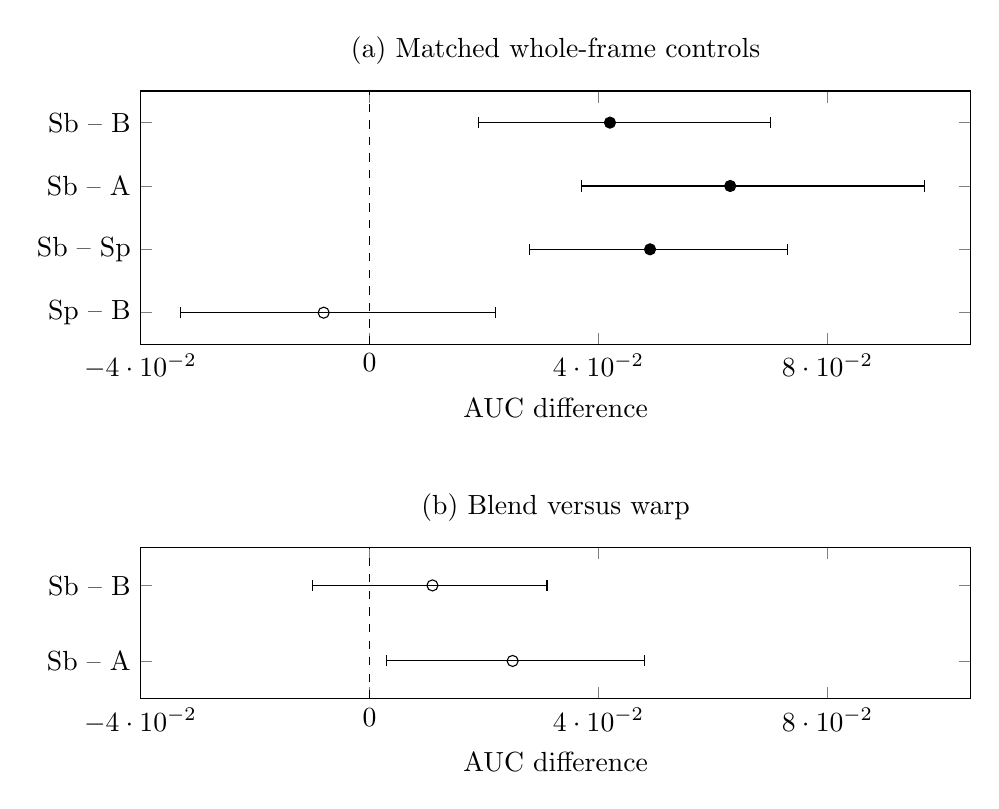
\begin{tikzpicture}
\begin{axis}[width=\linewidth,height=4.8cm,at={(0,0cm)},anchor=north west,scale only axis=false,title={(a) Matched whole-frame controls},xmin=-0.04,xmax=0.105,ymin=0.5,ymax=4.5,xtick={-0.04,0,0.04,0.08},xlabel={AUC difference},ytick={4,3,2,1},yticklabels={Sb -- B,Sb -- A,Sb -- Sp,Sp -- B}]
\addplot[dashed,mark=none] coordinates {(0,0.5) (0,4.5)};
\addplot[only marks,mark=*,error bars/.cd,x dir=both,x explicit] coordinates {(0.042,4) += (0.028000,0) -= (0.023000,0)};
\addplot[only marks,mark=*,error bars/.cd,x dir=both,x explicit] coordinates {(0.063,3) += (0.034000,0) -= (0.026000,0)};
\addplot[only marks,mark=*,error bars/.cd,x dir=both,x explicit] coordinates {(0.049,2) += (0.024000,0) -= (0.021000,0)};
\addplot[only marks,mark=o,error bars/.cd,x dir=both,x explicit] coordinates {(-0.008,1) += (0.030000,0) -= (0.025000,0)};
\end{axis}
\begin{axis}[width=\linewidth,height=3.5cm,at={(0,-5.8cm)},anchor=north west,scale only axis=false,title={(b) Blend versus warp},xmin=-0.04,xmax=0.105,ymin=0.5,ymax=2.5,xtick={-0.04,0,0.04,0.08},xlabel={AUC difference},ytick={2,1},yticklabels={Sb -- B,Sb -- A}]
\addplot[dashed,mark=none] coordinates {(0,0.5) (0,2.5)};
\addplot[only marks,mark=o,error bars/.cd,x dir=both,x explicit] coordinates {(0.011,2) += (0.020000,0) -= (0.021000,0)};
\addplot[only marks,mark=o,error bars/.cd,x dir=both,x explicit] coordinates {(0.025,1) += (0.023000,0) -= (0.022000,0)};
\end{axis}
\end{tikzpicture}

\fi
\caption{Development ranking gains. Top: two-person versus same-person whole-frame morphs, $D$-stratified, on development plus 80 person-overlap-screened hosts (seeds 408--412). Bottom: face-plus-halo blend-versus-warp diagnostic on FFHQ (seeds 403--407). Bars are 95\% component/block bootstrap intervals conditional on networks, not joint seed-and-host intervals. Filled/open points denote registered present/inconclusive verdicts. Panels use different data and resampling schemes.}
\label{fig:paired_evidence}
\end{figure}

\paragraph{Count-balanced follow-up.}
The post-freeze, development- and MAD22-informed follow-up reads all 30 networks (Sb, B, Sp, SpV, BN, BV; seeds 408--412), with no dropped seeds. Table~\ref{tab:count_balanced} reports its four registered outcomes. Primary OpenCV whole-frame ranking uses $D$-stratification on 100 development plus 80 screened test hosts; two-person whole-frame positives occur in training, but same-person whole-frame negatives do not. Secondary splice ranking uses the 80 screened hosts, unstratified as fixed before the read. Its 2,000 draws are all usable, unlike the stratified secondary diagnostic (37.7\% unreadable); primary stratification loses no draws. Both use paired host--partner component bootstraps (151/51 components), conditional on the five trained networks, without seed resampling.

\begin{table}[t]
\centering\small
\caption{Count-balanced development evidence: mean AUC differences and conditional 95\% component-bootstrap intervals. Positive-seed counts retain all five seeds.}
\label{tab:count_balanced}
\begin{tabular}{lccc}
\toprule
Pair & Gain & 95\% interval & Seeds $>0$ \\
\midrule
\multicolumn{4}{l}{Primary: whole-frame, $D$-stratified} \\
Sb $-$ SpV & +0.0481 & [0.0269, 0.0722] & 5/5 \\
BN $-$ BV & $-$0.0030 & [$-$0.0089, 0.0045] & 1/5 \\
\midrule
\multicolumn{4}{l}{Secondary: face splices, unstratified} \\
Sb $-$ SpV & +0.0818 & [0.0535, 0.1083] & 5/5 \\
BN $-$ BV & $-$0.0247 & [$-$0.0455, $-$0.0050] & 0/5 \\
\bottomrule
\end{tabular}
\end{table}

Sb--SpV supports replacing repeated native negatives with matched negatives plus 312 additional unique images in the full recipe. BN--BV lacks the registered $+0.03$ benefit on both outcomes; this is not equivalence to zero. Its adverse secondary effect contradicts the expected benefit: the 95\% interval is negative, but the 99.5\% sensitivity interval $[-0.0538,0.0031]$ crosses zero. Sb--SpV remains positive at 99.5\% on both outcomes; these sensitivities are not a familywise correction. Descriptive differences between pair effects are $+0.0511$ primary and $+0.1064$ secondary, with no interaction interval or significance test. Positive examples match only within pairs, so these differences do not isolate a universal requirement for splice positives. Independent numerical reconstruction exactly matched all 166 checks for the four outcomes; this verifies arithmetic, not external generalization.
% Sources: experiments/reviews/REVIEW_AB1_BATCHC_OPENCODE_20261114.md (full review);
% experiments/reviews/REVIEW_AB1_BATCHC_INDEPENDENT_REPRODUCTION_20261114.md (four-outcome reproduction).
% Reviewed output SHA256 9b73b148c57b9dbfbfdf60da2360aa9825ac7ddd8c42a94cd2fe137e21c802ea.
% Independent comparison SHA256 1b5a789ba01666c3c91e619c0049371ffcb85a1664536e23948461be8dc21bb7.
% Exact primary Sb-SpV +.048098592 [.026893408,.072238231]; BN-BV -.002992958 [-.008883478,.004497694].
% Exact secondary Sb-SpV +.081781250 [.053514957,.108347349]; BN-BV -.024656250 [-.045510204,-.005024836].

\paragraph{Storage sensitivity.}
Paired storage perturbations increase genuine false alarms by 26.5--38.5 percentage points for A at the trained small-image size, versus 0--4.5 points for Sb. At the untrained size, the corresponding ranges are 5.5--15.2 and 0--2.1 points. However, the registered test combines flag-rate and two-sided score-movement bounds. Sb passes five of five seeds at the trained size but only three at the untrained size: two failures arise from score movement toward genuine. The overall verdict is therefore inconclusive. We report attenuation of storage-induced false alarms, not removal of the shortcut.
% Source: AB1 result, registered R1 verdict and C2P per-seed rows.

\subsection{Development-exposed benchmark comparison}
\label{sec:mad22_results}
Table~\ref{tab:mad22_results} reports the frozen Sb networks on corrected MAD22~\cite{huber2022synmad}. No method met the registered freeze rule; the authors froze Sb by decision before these networks were benchmark-scored. The deciding endpoint was changed before that read from development-threshold errors to EER, because the training-source threshold flagged 96--98\% of unseen-source genuine photos. Its recipe was chosen after MAD22 results from earlier seeds were available; seeds 403--407 were new to benchmark evaluation. The genuine side comprises 204 FRLL photographs~\cite{debruine2017frll}. This is consequently a development-exposed benchmark evaluation, not an independent identity-level confirmation on FRLL. Released detectors are compared at their better raw-genuine or aligned-history form; SelfMAD's~\cite{ivanovska2025selfmad} raw form has the lowest four-family point mean among MADation B/16, MADation L/14, MixFaceNet-MAD and SelfMAD, each in raw-genuine and history-matched forms. This comparator is held fixed in bootstrap draws; it is not selected separately for each table row.
% Sources: experiments/FINAL_sealed-benchmark-read/result.md, labels and primary endpoint; prereg.md C1--C3 (freeze and endpoint amendments).

\begin{table}[t]
\centering\small
\caption{Corrected MAD22 EER (\%), lower is better. Sb uses the registered history-matched form and is averaged over five seeds. SelfMAD uses raw genuine photographs. MAD22 influenced recipe development.}
\label{tab:mad22_results}
\begin{tabular}{lrr}
\toprule
Family ($n$ morphs) & Sb & SelfMAD \\
\midrule
OpenCV (984) & 2.26 & 1.02 \\
Webmorph (500) & 10.39 & 13.73 \\
MIPGAN-I (1,000) & 0.57 & 2.45 \\
MIPGAN-II (999) & 0.28 & 1.70 \\
\midrule
Four-family mean & 3.37 & 4.72 \\
Landmark-only mean & 6.32 & 7.37 \\
\bottomrule
\end{tabular}
\end{table}

The four-family difference is $-1.4$ percentage points, with a two-level 95\% interval of $[-3.51,0.98]$. Each of 2,000 paired bootstrap draws resamples the 102 contributor persons and five seed indices. A genuine photo receives its person's multinomial count; a morph receives the product of both contributors' counts. Common draws serve all detectors and families. The registered one-point non-inferiority criterion narrowly passes: its bootstrap tail probability is 0.02499 against 0.025; one additional exceedance among 2,000 replicates changes the verdict. Superiority is not established. The landmark-only difference is $-1.0$ points $[-4.7,3.0]$ and is not separated. Half of the primary average comprises GAN families whose identity specificity remains unresolved by our rendering controls. FaceMorpher was excluded from this endpoint because morph-free networks achieve zero EER on that cell. Finally, EER is not the fixed-threshold error: Webmorph attack misses at the own rule range from 24--58\%, while genuine false alarms range from 0--2.5\%. These results support competitive discrimination alongside, rather than proof against, remaining shortcuts.


\section{Discussion and Limitations}
\paragraph{Mechanism and intervention.}
Morph-free benchmark separation and one-photo rendering responses establish processing sensitivity, not the absence of useful identity information or a common mechanism across detectors. Count-balanced gains in the full recipe control rows, classes and positive repetition within pairs, but matched-negative content remains confounded with 312 additional unique images. Absent registered benefit without splice positives is neither zero equivalence nor an interaction test.

\paragraph{Exposure and uncertainty.}
MAD22 informed development; new seeds do not restore independence. Its 204 FRLL photographs create exposure relevant to later FRLL-Morphs evaluation, which is not reported here. Component-only intervals condition on fitted networks and do not capture arbitrary retraining variability; dependence also limits effective sample size. No untouched-benchmark superiority is established.

\paragraph{Control validity and operation.}
Same-person manipulations test contributor dependence, not document acceptability. Blanking shifts the distribution and increases warp-only flags; in-domain simple-cue learners are explanatory references, not matched generalization competitors. Finite controls cannot establish universal shortcut freedom. Report ranking and perturbation responses alongside family-level attack misses and genuine false alarms: suppressing artifact responses is useful only if attack sensitivity is retained.

\section{Conclusion}
Single-image morph detection requires evidence beyond morph-versus-photo separation. Morph-free training and single-photo reconstruction controls show why strong benchmark performance can coexist with unresolved processing explanations. Our controlled comparisons expose these explanations, and matched-control training improves selected development contrasts while attenuating storage-induced false alarms. The remaining rendering response and inconclusive blend-control advantage define the next scientific challenge: preserving attack detection while demonstrating transfer under controls that increasingly constrain non-identity explanations.

\section*{LLM Usage Statement}
OpenAI Codex assisted with organizing experiment records and auditing evidence; proposing experiments; preparing training, analysis and infrastructure code; coordinating experiments; literature research; manuscript drafting and revision; and preparing figures derived from experimental data. This is a draft disclosure of the confirmed Codex scope. Historical Claude and OpenCode records were imported as context; the authors must verify the full historical tool usage and its extent, and finalize this statement before submission.

{\small\bibliographystyle{ieeenat_fullname}\bibliography{references}}
\end{document}
